%% =====================================================================
%%  CAPITULO 8 - EXPERIMENTOS E RESULTADOS
%% =====================================================================

\chapter{Experimentos e Resultados}
\label{cap:resultados}

Este capítulo reporta o protocolo de verificação e os resultados obtidos.
Reportam-se apenas resultados efetivamente observados; o que não foi verificado
está enumerado na Seção~\ref{sec:res-nao-verificado}.

\section{Protocolo de verificação}
\label{sec:res-protocolo}

A verificação executou os doze critérios de aceitação do Quadro~\ref{qua:ca},
mais uma medição quantitativa do intervalo entre passos de simulação. Para cada
critério, o resultado foi classificado como satisfeito, não satisfeito ou não
verificável. A classificação não admitiu valor intermediário.

Dois procedimentos foram usados. A inspeção estática verificou propriedades
estruturais que não dependem de execução, por busca textual no artefato. A
execução observada verificou comportamento, por automação de navegador com envio
de eventos e leitura do estado observável da página, incluindo amostragem de
pixels da superfície de desenho.

A opção por observação externa, sem instrumentar o produto, é deliberada. Um
teste que exige alterar o código para expor o estado interno mede o código
alterado, não o código entregue. A leitura de pixels contorna essa objeção: ela
observa exatamente o que o usuário vê.

\section{Resultados por critério de aceitação}
\label{sec:res-ca}

A Tabela~\ref{tab:ca-resultados} consolida os resultados. Cada linha registra o
critério, o instrumento usado, a observação e o resultado.

\begin{table}[htb]
	\caption{Resultado da verificação por critério de aceitação}
	\label{tab:ca-resultados}
	\centering
	\scriptsize
	\begin{tabularx}{\textwidth}{@{}p{1.3cm} p{2.1cm} X c@{}}
		\toprule
		\textbf{CA} & \textbf{Instrumento} & \textbf{Observação registrada} & \textbf{Resultado} \\
		\midrule
		CA-001 & Inspeção estática & Busca por referências de rede, de script e de estilo retornou vazio; exatamente um bloco de estilo e um de script & Satisfeito \\
		\addlinespace
		CA-002 & Execução observada & Entrada ``direita'' seguida de ``esquerda'': o jogador manteve o sentido e encerrou por colisão com a borda direita & Satisfeito \\
		\addlinespace
		CA-003 & Execução observada & Agente de teste orientado por busca em largura: pontuação passou de 0 para 10 após consumo & Satisfeito \\
		\addlinespace
		CA-004 & Execução observada & 25 amostras da célula do alvo; nenhuma sobreposição com células de corpo & Satisfeito \\
		\addlinespace
		CA-005 & Execução observada & Colisão com a borda: título da sobreposição passou a ``Fim de jogo'' e botão de reinício exibido & Satisfeito \\
		\addlinespace
		CA-006 & Execução observada & Após crescimento, giro fechado em quatro células encerrou a partida com a cabeça em célula interior (6,6), longe das bordas & Satisfeito \\
		\addlinespace
		CA-007 & Execução observada & Chave de armazenamento local com valor ``10'' e, em execução posterior, ``100''; valor mantido após recarregar & Satisfeito \\
		\addlinespace
		CA-008 & Execução observada & Acionamento do botão superior moveu a cabeça de (11,11) para (12,9) & Satisfeito \\
		\addlinespace
		CA-009 & Execução observada & Sobreposição visível antes; oculta após a primeira direção válida & Satisfeito \\
		\addlinespace
		CA-010 & Execução observada & Estado ``Pausado'': cabeça imóvel em (12,9) por 600\,ms; retomada ocultou a sobreposição & Satisfeito \\
		\addlinespace
		CA-011 & Execução observada & Registro de erros e exceções do console vazio ao longo de todas as execuções & Satisfeito \\
		\addlinespace
		CA-012 & Medição & Intervalo médio 133\,ms com pontuação abaixo de 40 e 105\,ms com pontuação igual ou superior a 80 (Seção~\ref{sec:res-velocidade}) & Satisfeito \\
		\bottomrule
	\end{tabularx}
	\legend{Fonte: elaborado pelo autor (2026) a partir de \texttt{docs/05-testing/snake-game-evidence.md}.}
\end{table}

Substituindo na Equação~(\ref{eq:cobertura}), obtém-se

\begin{equation}
	A = \frac{12}{12} = 1{,}00,
	\label{eq:resultado-cobertura}
\end{equation}

\noindent isto é, todos os critérios de aceitação declarados foram satisfeitos.
O alcance dessa afirmação está limitado ao que está escrito na
Seção~\ref{sec:res-nao-verificado}.

\section{Cobertura de rastreabilidade}
\label{sec:res-rastreabilidade}

Além do resultado por critério, mediu-se a cobertura de rastreabilidade: a fração
de requisitos que possui critério de aceitação associado. A
Tabela~\ref{tab:cobertura-req} apresenta o resultado, obtido por contagem direta
na especificação.

\begin{table}[htb]
	\caption{Cobertura de rastreabilidade por classe de requisito}
	\label{tab:cobertura-req}
	\centering
	\footnotesize
	\begin{tabularx}{\textwidth}{@{}p{3.4cm} c c c c@{}}
		\toprule
		\textbf{Classe} & \textbf{Total} & \textbf{Com CA} & \textbf{Parcial} & \textbf{Cobertura} \\
		\midrule
		Requisitos funcionais & 15 & 11 & 1 & 73,3\,\% \\
		\addlinespace
		Requisitos não funcionais & 9 & 2 & 0 & 22,2\,\% \\
		\addlinespace
		\textbf{Total} & \textbf{24} & \textbf{13} & \textbf{1} & \textbf{54,2\,\%} \\
		\bottomrule
	\end{tabularx}
	\legend{Fonte: elaborado pelo autor (2026), por contagem em \texttt{spec.md}.
	``Parcial'' indica requisito coberto apenas em parte pelo critério associado.}
\end{table}

Os requisitos funcionais sem critério dedicado são \texttt{FR-002} (uso da
superfície de desenho), \texttt{FR-009} (exibição do placar) e \texttt{FR-014}
(laço de animação). \texttt{FR-011} está parcialmente coberto: o critério
\texttt{CA-005} verifica a exibição da tela de fim de jogo, mas não o
funcionamento do botão de reinício, que foi observado empiricamente sem
critério correspondente.

A assimetria entre as duas classes é o achado mais informativo desta seção. A
cobertura de requisitos funcionais é de 73,3\,\%, enquanto a de requisitos não
funcionais é de 22,2\,\%. A diferença não é acidental: requisitos funcionais
descrevem comportamento observável e convertem-se naturalmente em teste;
requisitos não funcionais, quando enunciados como atributos, não geram teste
óbvio --- e, sem teste, não geram critério. A consequência é que sete dos nove
requisitos não funcionais ficaram fora de qualquer portão de aceitação.

Esse resultado não decorre do framework, e sim da especificação que o framework
aceitou como válida. O portão G1 exige que existam requisito \emph{e} critério
antes da implementação; ele não exige que \emph{todo} requisito tenha critério.
Essa é uma lacuna do portão, identificada por autocrítica e discutida na
Seção~\ref{sec:disc-lacunas-do-gate}.

\section{Verificação de propriedades estruturais}
\label{sec:res-estruturais}

A inspeção estática produziu as seguintes observações concretas:

\begin{itemize}
	\item um único arquivo, com exatamente um bloco de estilo e um bloco de script;
	\item nenhuma referência de rede a script, estilo, fonte ou imagem em qualquer ponto do artefato;
	\item sete campos no objeto de configuração, com valores idênticos aos especificados na Tabela~\ref{tab:constantes};
	\item ausência de temporizador de intervalo fixo para a simulação, conforme \texttt{CON-004};
	\item treze seções comentadas, conforme \texttt{NFR-005}.
\end{itemize}

Essas observações sustentam \texttt{CA-001} e as restrições \texttt{CON-001} a
\texttt{CON-004}. Elas são o tipo de evidência mais barato de produzir e o mais
barato de reproduzir, porque não depende de ambiente de execução.

\section{Medição do intervalo entre passos}
\label{sec:res-velocidade}

A única medição quantitativa de comportamento contínuo foi o intervalo entre
passos de simulação, previsto pela Equação~(\ref{eq:velocidade-simplificada}) e
exigido por \texttt{FR-015} e \texttt{CA-012}.

\subsection{Procedimento}
\label{subsec:res-procedimento}

Um agente de teste jogou a partida de forma autônoma, localizando o alvo e a
cabeça por amostragem de pixels e escolhendo o caminho mais curto por busca em
largura sobre a grade livre. A cada mudança de posição da cabeça, registrou-se um
par (instante, pontuação corrente). A partida foi conduzida até a pontuação de
100 pontos, sem encerramento por colisão.

Foram amostrados 184 movimentos. Os intervalos foram agrupados em duas faixas de
pontuação e a média foi calculada pela Equação~(\ref{eq:intervalo-medio}).

\subsection{Resultado}
\label{subsec:res-resultado-velocidade}

A Tabela~\ref{tab:velocidade} confronta o valor medido com o intervalo previsto
pelo modelo da Equação~(\ref{eq:velocidade-simplificada}) para a faixa
correspondente.

\begin{table}[htb]
	\caption{Intervalo médio entre passos medido e previsto, por faixa de pontuação}
	\label{tab:velocidade}
	\centering
	\footnotesize
	\begin{tabularx}{\textwidth}{@{}p{3.2cm} c c c c@{}}
		\toprule
		\textbf{Faixa de pontuação} & \textbf{Média medida} & \textbf{Previsto (mín.)} & \textbf{Previsto (máx.)} & \textbf{Coerente} \\
		\midrule
		Abaixo de 40 pontos & 133\,ms & 128\,ms & 140\,ms & Sim \\
		\addlinespace
		80 pontos ou mais & 105\,ms & 100\,ms & 108\,ms & Sim \\
		\bottomrule
	\end{tabularx}
	\legend{Fonte: elaborado pelo autor (2026). Previsto pela Equação~(\ref{eq:velocidade-simplificada})
	nos extremos de cada faixa. Número de amostras por faixa não retido no registro de evidência --- ver P-11.}
\end{table}

Os dois valores medidos caem dentro do intervalo previsto para a faixa
correspondente, com desvio de 1\,ms em relação ao ponto médio de cada intervalo
previsto. A diferença entre as duas faixas é de 28\,ms, contra 28\,ms previstos
na comparação dos pontos médios (134\,ms e 104\,ms). A direção da variação ---
intervalo menor com pontuação maior --- coincide com a exigida por
\texttt{FR-015}.

Três advertências sobre a interpretação acompanham esse resultado.

\textbf{A medição é um limite superior.} O ciclo de observação introduz atraso
positivo: o instante registrado é posterior ao instante real da mudança de
posição. Os valores medidos não devem ser lidos como estimativas do parâmetro
\texttt{stepMs}, e sim como valores comparáveis entre si.

\textbf{A média de faixa pressupõe distribuição aproximadamente uniforme da
pontuação dentro da faixa.} Essa suposição não foi verificada. Ela é plausível
para a faixa alta, que cobre dois itens consumidos, mas não foi controlada.

\textbf{A amostra é única.} Não houve repetição do experimento, e portanto não há
intervalo de confiança nem teste de hipótese. A conclusão sustentada é de
coerência entre o medido e o previsto, não de significância estatística.

A Figura~\ref{fig:velocidade} representa a curva prevista pela especificação e
posiciona os dois valores medidos. A curva é \emph{modelo}, não medição; os dois
pontos são \emph{medição}, não modelo. A distinção é mantida visualmente e na
legenda.

%% ---------------------------------------------------------------------
%%  FIGURA - Curva do modelo de velocidade e pontos medidos (DG-11)
%%
%%  ATENCAO METODOLOGICA: a curva e o MODELO definido na especificacao
%%  (Equacao da secao 6.8). Os dois pontos sao MEDICOES da secao 8.5.
%%  Modelo e medicao nunca sao misturados nesta figura.
%% ---------------------------------------------------------------------
\begin{figure}[htb]
	\caption{Curva do modelo de velocidade da especificação e os dois valores medidos}
	\label{fig:velocidade}
	\centering
	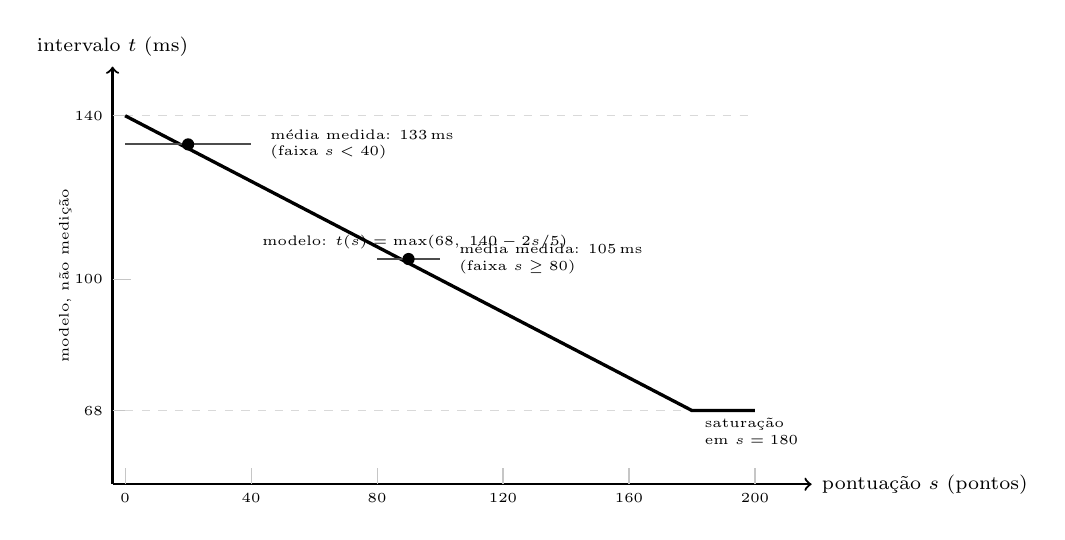
\begin{tikzpicture}[
			font=\scriptsize,
			x=0.040cm,
			y=0.052cm
		]

		% ---- eixos -----------------------------------------------------
		\draw[->, thick] (-4,50) -- (218,50) node[right] {pontuação $s$ (pontos)};
		\draw[->, thick] (-4,50) -- (-4,152) node[above, align=center] {intervalo $t$ (ms)};

		% ---- grade e marcas -------------------------------------------
		\foreach \x in {0,40,80,120,160,200} {
				\draw[gray!45, thin] (\x,50) -- (\x,54);
				\node[below, font=\tiny] at (\x,50) {\x};
			}
		\foreach \y in {68,100,140} {
				\draw[gray!45, thin] (-4,\y) -- (2,\y);
				\node[left, font=\tiny] at (-4,\y) {\y};
			}
		\draw[gray!30, dashed, thin] (0,68) -- (200,68);
		\draw[gray!30, dashed, thin] (0,140) -- (200,140);

		% ---- curva do modelo t(s) = max(68, 140 - 2s/5) ---------------
		\draw[very thick] (0,140) -- (180,68) -- (200,68);
		\node[above, font=\tiny, align=center] at (92,105) {modelo: $t(s) = \max(68,\; 140 - 2s/5)$};
		\node[right, font=\tiny, align=left] at (181,63) {saturação\\ em $s = 180$};

		% ---- faixas medidas ------------------------------------------
		% faixa baixa: pontuacao < 40, media medida 133 ms
		\draw[thick, black!70] (0,133) -- (40,133);
		\fill[black] (20,133) circle (2.2pt);
		\node[right, font=\tiny, align=left] at (43,133) {média medida: 133\,ms\\(faixa $s < 40$)};

		% faixa alta: pontuacao >= 80, media medida 105 ms
		\draw[thick, black!70] (80,105) -- (100,105);
		\fill[black] (90,105) circle (2.2pt);
		\node[right, font=\tiny, align=left] at (103,105) {média medida: 105\,ms\\(faixa $s \geq 80$)};

		% ---- anotacao do eixo y --------------------------------------
		\node[rotate=90, anchor=south, font=\tiny] at (-14,101) {modelo, não medição};
	\end{tikzpicture}
	\legend{Fonte: elaborado pelo autor (2026). A \textbf{curva} é o modelo declarado na especificação
	(Equação~(\ref{eq:velocidade-simplificada})), não uma medição. As \textbf{barras horizontais} são as
	faixas de pontuação sobre as quais cada média foi calculada, e os \textbf{círculos} são as médias
	medidas na Seção~\ref{sec:res-velocidade}. Os valores medidos incluem atraso positivo do ciclo de
	observação e não devem ser lidos como estimativas do parâmetro \texttt{stepMs}.}
\end{figure}


\section{Comportamentos observados sem critério correspondente}
\label{sec:res-extras}

Durante a verificação, quatro comportamentos foram observados mas não possuem
critério de aceitação associado. Registrá-los é obrigatório do ponto de vista da
integridade: são resultados, ainda que não estivessem previstos como testes.

\begin{enumerate}
	\item O reinício por tecla de confirmação na tela de fim de jogo restaura o estado e inicia a movimentação.
	\item O reinício por tecla R restaura a partida a partir de qualquer estado ativo.
	\item A perda de foco da janela provoca pausa automática.
	\item Girando em quadrado com comprimento quatro, o jogador sobrevive; a partir de comprimento cinco, colide consigo mesmo. Esse comportamento é a consequência observável de ADR-004 e confirma materialmente o caso de borda~5.
\end{enumerate}

O item 4 é o de maior valor para o trabalho, porque converte uma decisão
arquitetural em comportamento observável e, portanto, em evidência. Ele mostra
que ADR-004 não é uma preferência de estilo: produz diferença verificável no
comportamento do produto para a mesma especificação de requisitos.

\section{O que não foi verificado}
\label{sec:res-nao-verificado}

A Tabela~\ref{tab:nao-verificado} enumera o que ficou fora da verificação. Nenhum
item foi preenchido por estimativa.

\begin{table}[htb]
	\caption{Itens não verificados e razão}
	\label{tab:nao-verificado}
	\centering
	\footnotesize
	\begin{tabularx}{\textwidth}{@{}p{4.6cm} X@{}}
		\toprule
		\textbf{Item} & \textbf{Razão} \\
		\midrule
		Controles de toque em dispositivo móvel físico & Verificado apenas por emulação de evento de apontador em navegador de desktop. A diretriz do framework estabelece que emulação não promove o nível de evidência. Pendência registrada no projeto como T-016. \\
		\addlinespace
		Consumo de memória e taxa de quadros & Não instrumentado. Nenhuma meta foi declarada na especificação, e portanto nenhum critério existe. \\
		\addlinespace
		Responsividade em todas as larguras de 320\,px a 1920\,px & Verificada por cálculo de caixa de layout em uma largura e por inspeção dos pontos de quebra; não amostrada em todas as larguras. \\
		\addlinespace
		Leitores de tela e tecnologias assistivas & A estrutura semântica foi inspecionada; não houve teste com leitor de tela real. \\
		\addlinespace
		Navegadores alternativos ao motor Chromium & Não testado. A especificação não declara matriz de compatibilidade. \\
		\addlinespace
		Comportamento sob armazenamento local indisponível & O tratamento de exceção existe por inspeção, mas o cenário não foi reproduzido em execução. \\
		\bottomrule
	\end{tabularx}
	\legend{Fonte: elaborado pelo autor (2026).}
\end{table}

\section{Síntese do capítulo}
\label{sec:res-sintese}

A verificação produziu três resultados: doze de doze critérios de aceitação
satisfeitos, uma cobertura de rastreabilidade de 54,2\,\% sobre o conjunto de
requisitos, com forte assimetria entre requisitos funcionais (73,3\,\%) e não
funcionais (22,2\,\%), e uma medição de intervalo entre passos coerente com o
modelo da especificação em duas faixas de pontuação, com diferença de 28\,ms entre
elas. Seis itens permaneceram fora da verificação, e nenhum foi preenchido por
estimativa.
